\graphicspath{{content/chapters/5_design/figures/}}
\chapter{Design}
\label{chp:design}

\section{Variable Length Handling}
\label{sec:variable_length_handling}

For this project, only the clean and noisy pairs of audio files from the dataset are required. The transcript text files are ignored, as they are not relevant to the task. However, it is worth noting that such transcripts are highly valuable in other applications, such as training text-to-speech or speech recognition models. As highlighted in the dataset analysis in Section~\ref{sec:dataset_exploration}, the audio files vary in length. This poses a challenge for model training, as batch processing requires input tensors to have consistent dimensions.

To address this, several algorithms for handling variable-length audio inputs were explored. The most basic approach involves padding each audio file to match the length of the longest sample in the batch, typically by appending zeros to the end of shorter files. While this method is simple, it has significant drawbacks: excessive padding introduces unnecessary data that may act as noise during training, making it harder for the model to learn effectively. The greater the variation in input lengths, the more padding is required — which can negatively impact overall training performance.

\begin{figure}[h]
    \centering
    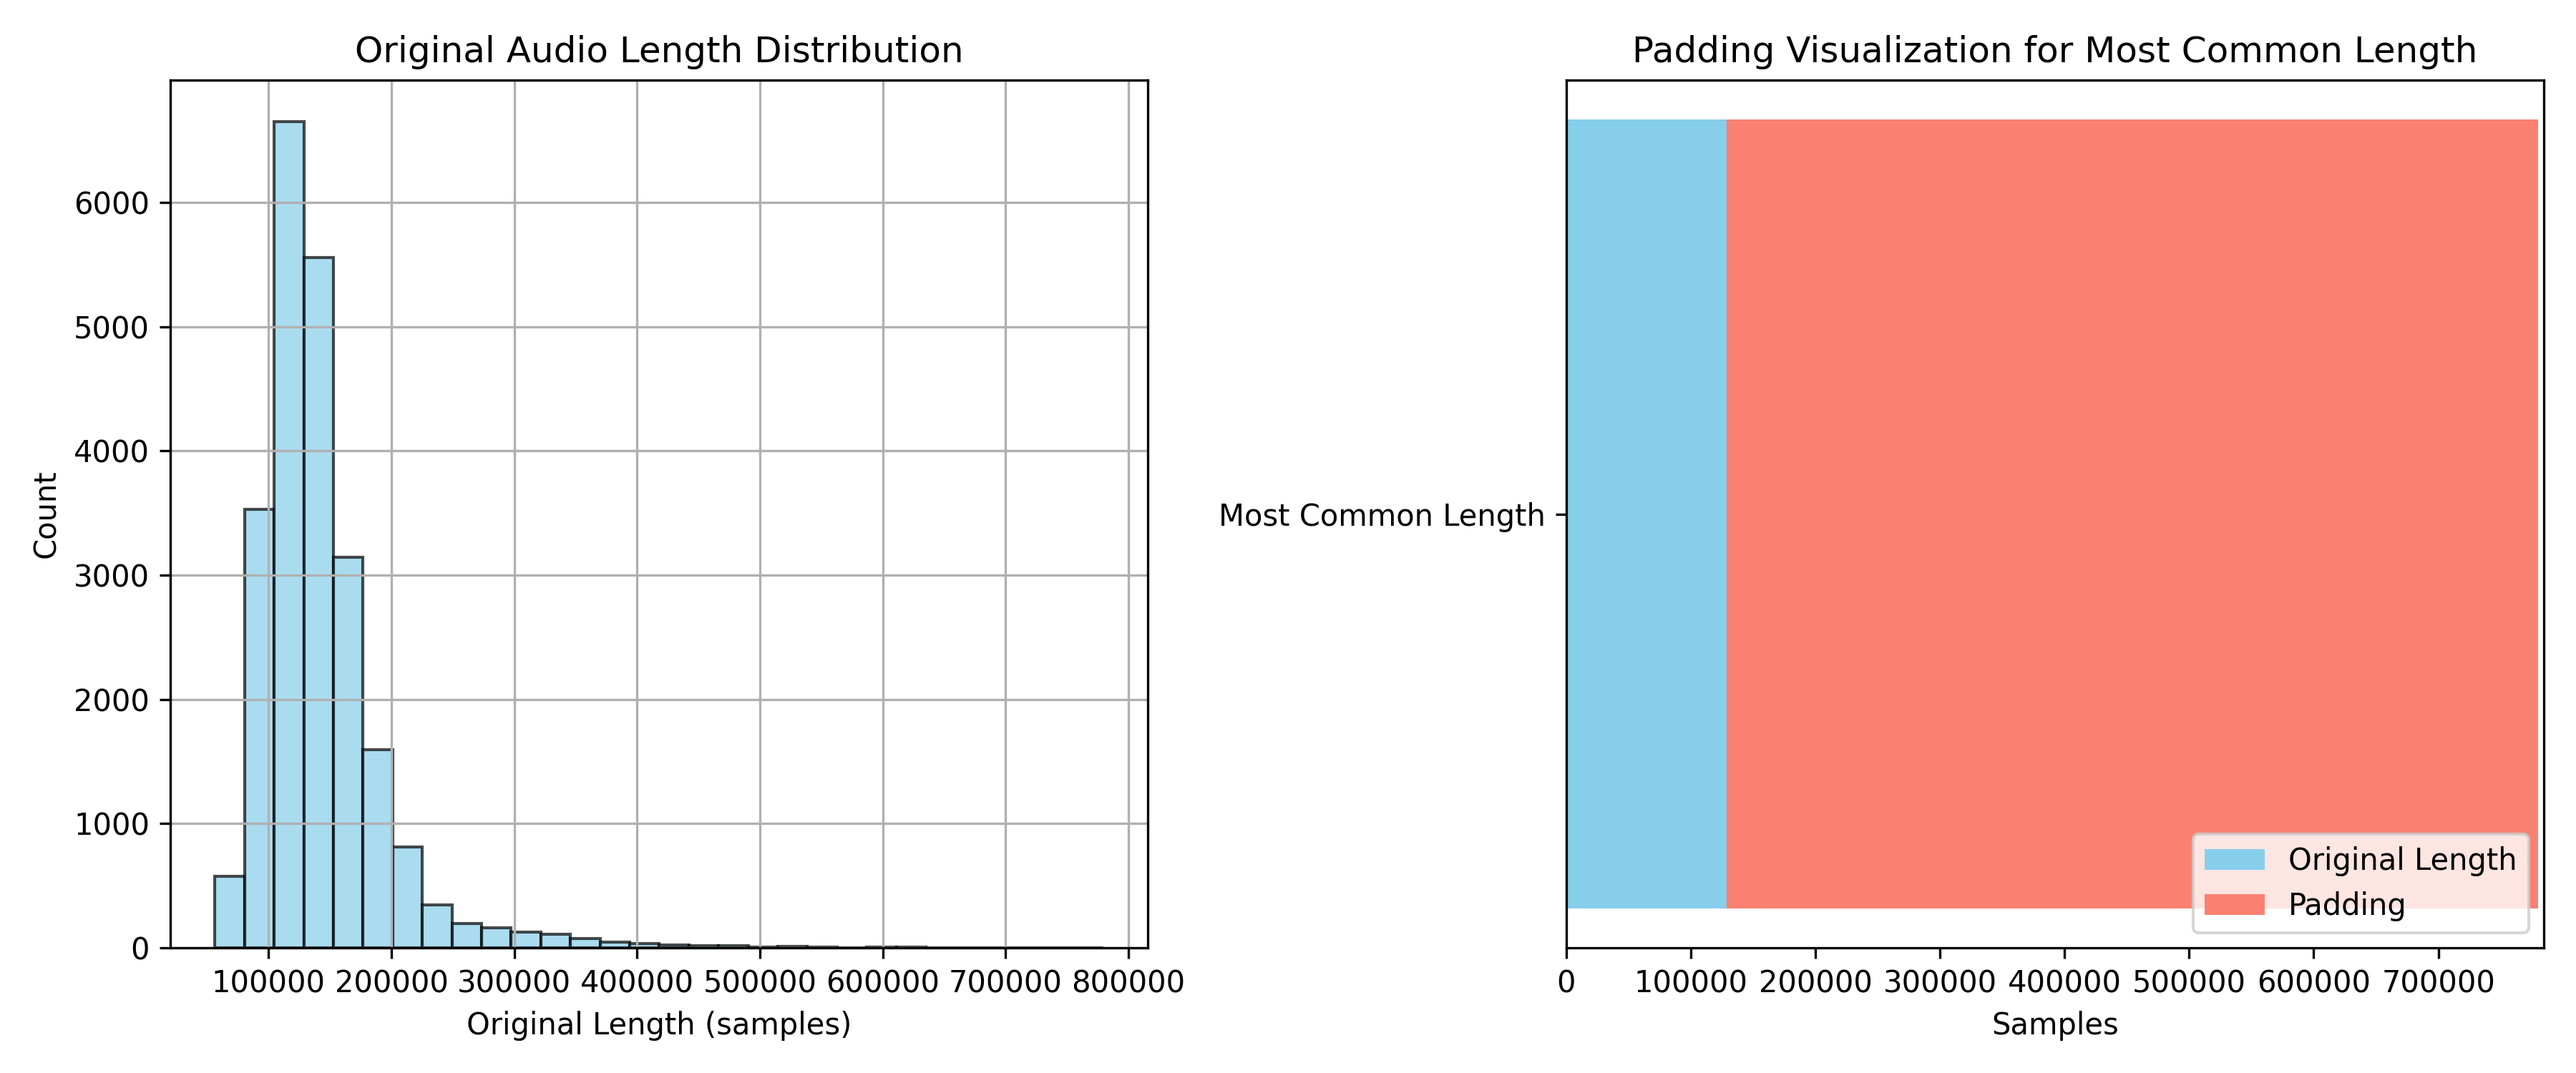
\includegraphics[width=\textwidth,keepaspectratio]{max_padding.png}
    \caption{\label{fig:max_padding}Illustration of maximum-length padding.}
\end{figure}

As shown in Figure~\ref{fig:max_padding}, the most common audio length is padded so heavily that the padding exceeds the actual content. This is far from ideal. To mitigate this issue, three different padding strategies were used. Each method aims to reduce the impact of excessive padding on model performance.

The first method is \textit{Static Bucketing}, which essentially groups audio files into predefined fixed-length buckets. Allowing the grouped files to require less unnecessary padding. The second method, \textit{Dynamic Bucketing}, builds on this by creating buckets dynamically based on the distribution of audio lengths, offering a more adaptive grouping approach. The third and final method introduced in Section~\ref{sec:pto_variable_length_sequences}. PTO enables dynamic padding within each batch and output truncation after inference, ensuring minimal distortion and preserving alignment with the original input lengths.

All three methods were implemented for testing and evaluation. Their role in the system design is critical, as they help ensure that the model can learn effectively without being hindered by dimensional mismatches or excessive zero-padding. Further details on the implementation of these methods are provided in Chapter~\ref{chp:implementation}, and their impact on model performance is discussed in Chapter~\ref{chp:evaluation}.

\section{Model Architecture}
\label{sec:model_architecture}

The model architecture forms the core of the system design, determining how the input is processed, how latent features are transformed, and how the output is reconstructed. The modular project structure facilitates the exploration of a range of neural network models, starting with a simple baseline and progressing to more advanced designs. The main concept of autoencoders for speech enhancement models has already been introduced in Section \ref{sec:machine_learning}. All models operate on spectrogram representations of audio, where the real and imaginary components are concatenated to form a two-channel input. Each network outputs a similarly formatted spectrogram, with values bounded to \([-1, 1]\) using a \texttt{Tanh} activation at the output. The most basic model defined in this work is a convolutional neural network (CNN) autoencoder.

\subsection{Convolutional Neural Network (CNN)}
\label{sec:cnn}

The CNN model implemented in this project serves as the baseline architecture. It is designed as a basic encoder-decoder model that operates directly on the real and imaginary components of the spectrogram, which are concatenated into a two-channel input. The encoder compresses the input using a series of three simple convolutional blocks, each consisting of a convolutional layer followed by a PReLU activation function. The encoder progressively reduces the spatial dimensions while increasing the depth of the feature maps, allowing the model to learn increasingly abstract representations of the input data.

\begin{figure}[h]
    \centering
    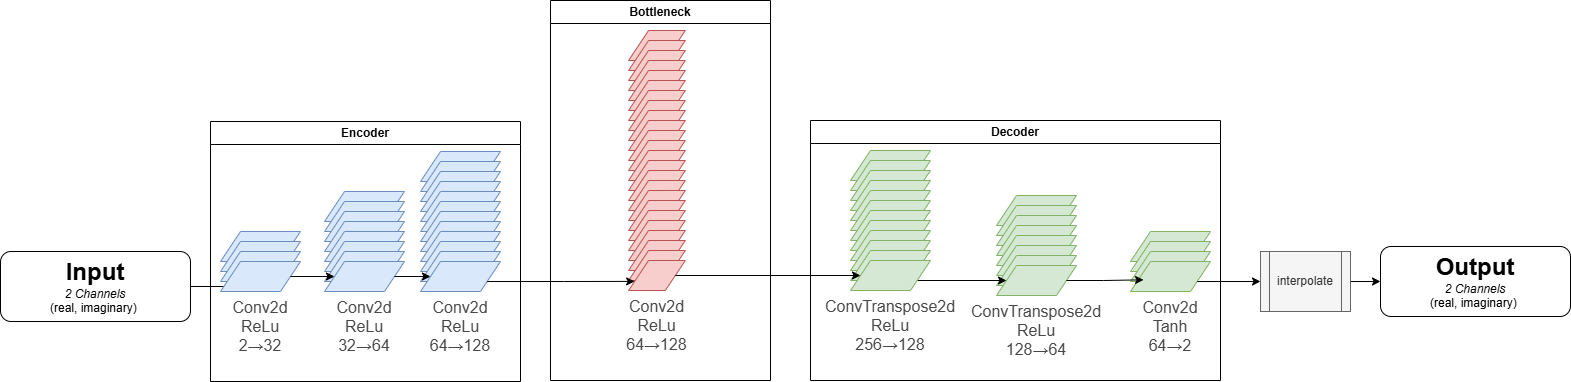
\includegraphics[width=\textwidth,keepaspectratio]{cnn.png}
    \caption{\label{fig:cnn}Basic CNN architecture.}
\end{figure}

The encoder then passes the compressed representation to the bottleneck layer, which is used to further transform the feature space and encourage the model to learn a more compact and expressive representation of the input. Bottleneck layers in machine learning architectures are often used to reduce the dimensionality of the latent representation, act as a regularizer, or increase non-linearity before reconstruction. In this implementation, the bottleneck is intentionally kept simple, consisting of a single additional convolutional layer with a higher channel depth (126 -> 256) followed by a PReLU activation function. This layer is placed outside of the encoder and decoder blocks to preserve architectural modularity and to isolate the representation-learning stage from the downsampling and upsampling operations. While not a traditional bottleneck in terms of dimensionality reduction, it acts as a feature transformer and deepens the network's capacity without affecting the input/output resolution.

Following the bottleneck, the decoder reconstructs the spectrogram from the transformed latent features. It mirrors the encoder structure by using two transposed convolutional layers (also known as deconvolution layers), each followed by a PReLU activation function. These layers progressively upsample the feature maps, restoring the spatial dimensions that were reduced during the encoding process. The decoder is responsible for reintroducing fine-grained details and structural patterns necessary to reconstruct a clean version of the original spectrogram from its compressed representation.

The final layer of the network is a standard convolutional layer that reduces the number of channels from 64 to 2, corresponding to the real and imaginary parts of the denoised spectrogram. This is followed by a \texttt{Tanh} activation function, which constrains the output values to the range \([-1, 1]\). This output range is especially useful when reconstructing signals via the inverse Short-Time Fourier Transform (iSTFT), promoting numerical stability and boundedness. This final output formatting is used consistently across all models described in this work.


While simple, this model plays a critical role in establishing a baseline performance level. It ensures that the overall system functions correctly while providing a reference point for evaluating the impact of architectural modifications. The CNN model is straightforward to implement and interpret, making it a suitable starting point for benchmarking and for guiding the development of more sophisticated architectures introduced in subsequent sections.

\subsection{Convolutional Encoder Decoder (CED)}
\label{sec:ced}

The Convolutional Encoder Decoder (CED) architecture implemented in this project is based on the model introduced by Park and Lee~\cite{park2017acoustic} and reviewed in Section~\ref{sec:fcns}. The CED follows a symmetric encoder-decoder structure designed for spectrogram enhancement, optimized for temporal feature extraction using frequency-preserving convolutional kernels. In this implementation, the real and imaginary components of the spectrogram are concatenated to form a two-channel input.


\begin{figure}[h]
    \centering
    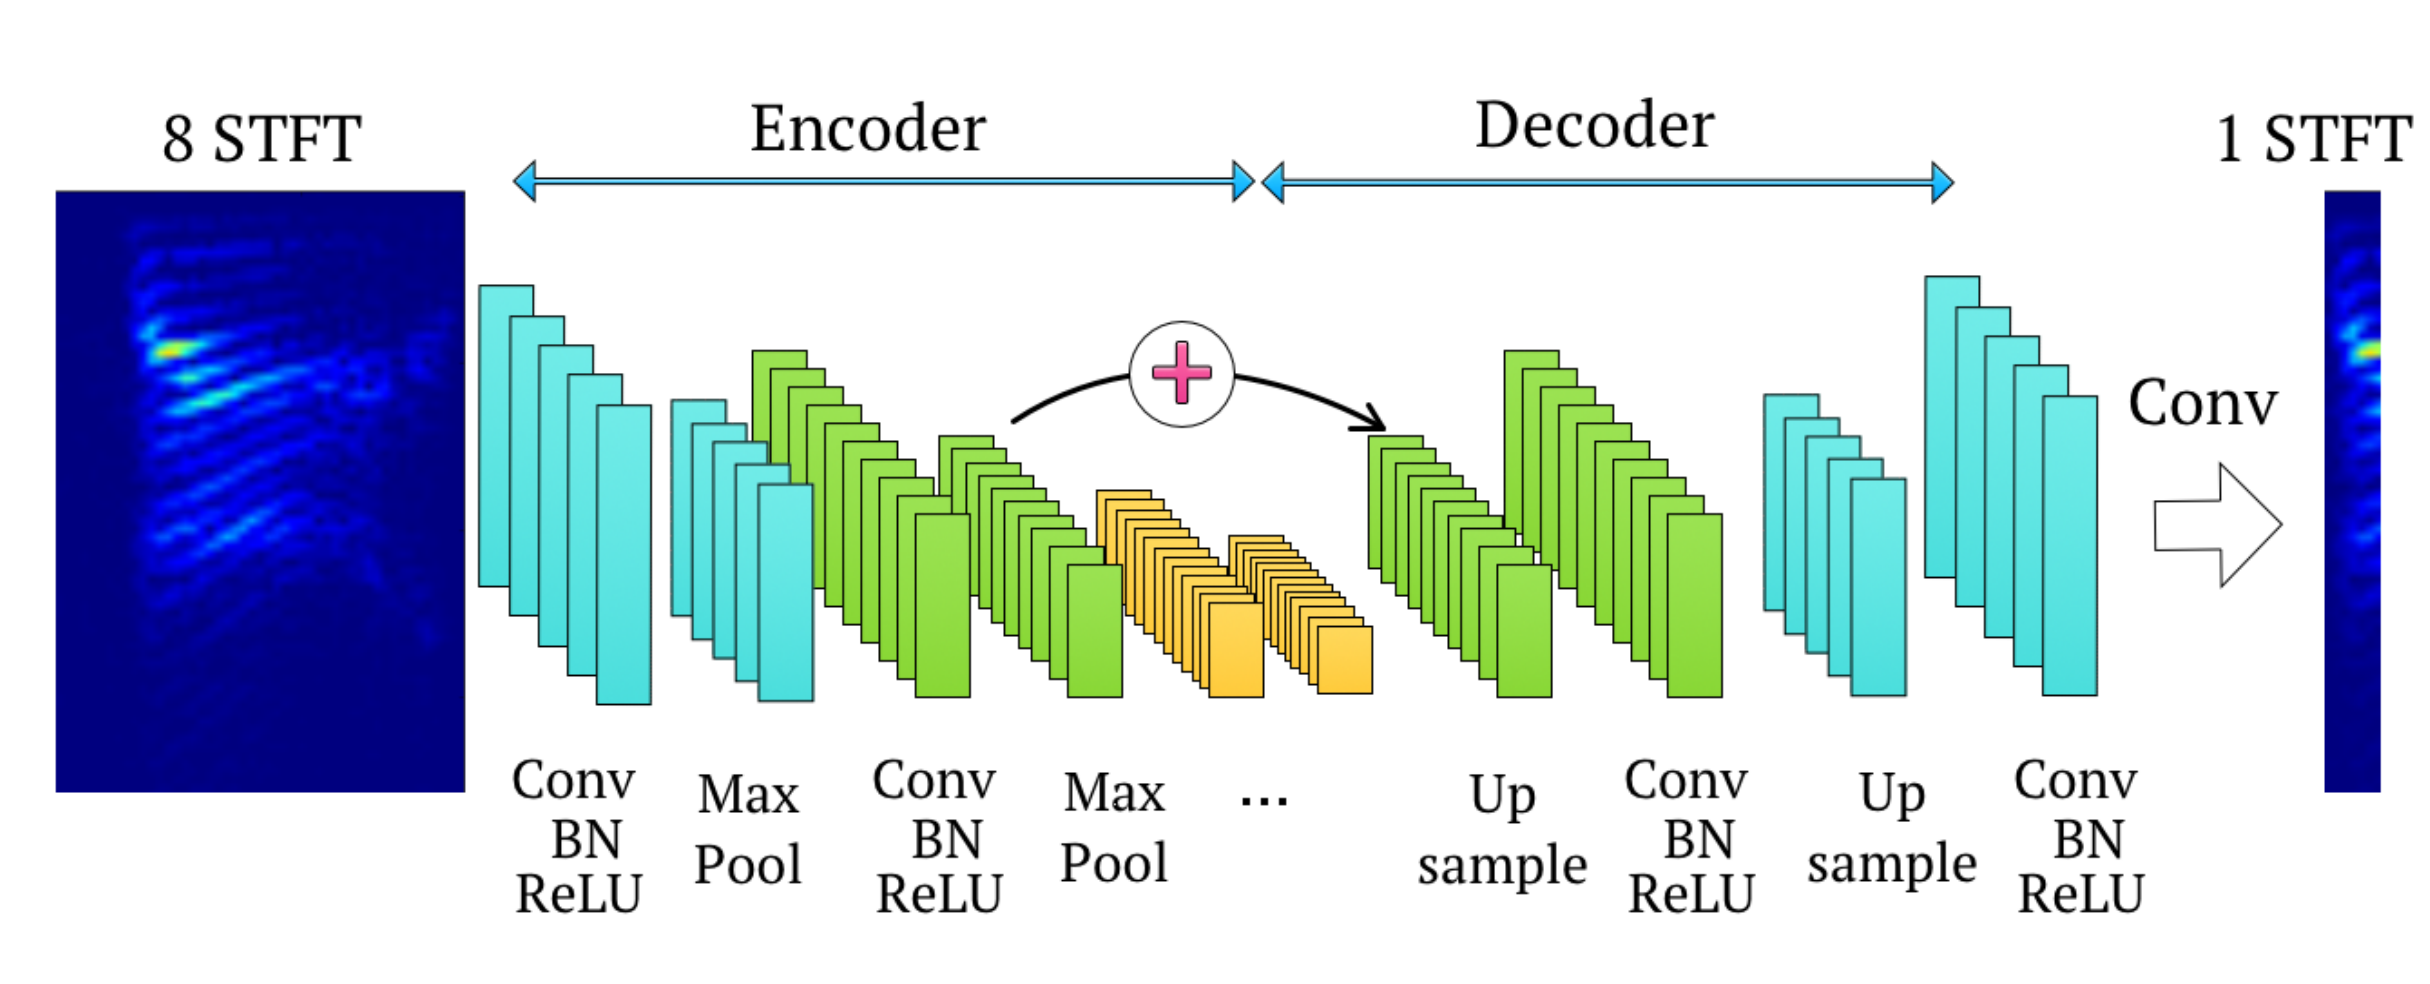
\includegraphics[width=\textwidth,keepaspectratio]{ced.png}
    \caption{\label{fig:ced}Convolutional Encoder Decoder (CED) Network\cite{park2017acoustic}.}
\end{figure}

The encoder is composed of five convolutional blocks. Each block consists of a convolutional layer with a tall vertical kernel (ranging from \(13 \times 1\) to \(5 \times 1\)), followed by batch normalization, a ReLU activation function, and a \(2 \times 1\) max pooling operation. These blocks progressively downsample the temporal resolution while preserving frequency content, allowing the model to focus on temporal patterns critical for speech structure. As the signal propagates through the encoder, the number of feature channels increases (from 12 up to 32), allowing for richer and more abstract representations to be learned.

In contrast to the baseline CNN, the CED model omits a distinct bottleneck layer. Instead, the compressed representation at the output of the encoder directly feeds into the decoder. The decoder mirrors the encoder using upsampling layers followed by convolution, batch normalization, and ReLU activation, progressively restoring the temporal resolution. A final convolutional layer with a large vertical kernel size of \(129 \times 1\) is used to project the output to two channels. The final activation and output formatting follow the same convention established in the CNN model.

By removing the bottleneck and relying on deeper convolutional transformations, the CED model allows for a smoother flow of information from input to output. Its symmetric structure and tailored kernel dimensions make it particularly well-suited for speech enhancement, as demonstrated in the original work by Park and Lee. In this project, the CED serves as a strong benchmark to evaluate the benefits of deeper temporal modeling compared to the simpler CNN baseline.

\subsection{Redundant Convolutional Encoder Decoder (R-CED)}
\label{sec:rced}

The Redundant Convolutional Encoder Decoder (R-CED) architecture implemented in this project builds upon the CED framework. Also introduced by Park and Lee~\cite{park2017acoustic} and discussed in Section~\ref{sec:fcns}. R-CED removes pooling and upsampling operations entirely, instead relying on redundant convolutional layers to maintain full temporal and frequency resolution throughout the network. In this implementation, the real and imaginary spectrogram components are again concatenated into a two-channel input, with the goal of preserving fine-grained spectro-temporal structures during enhancement.

\begin{figure}[h]
    \centering
    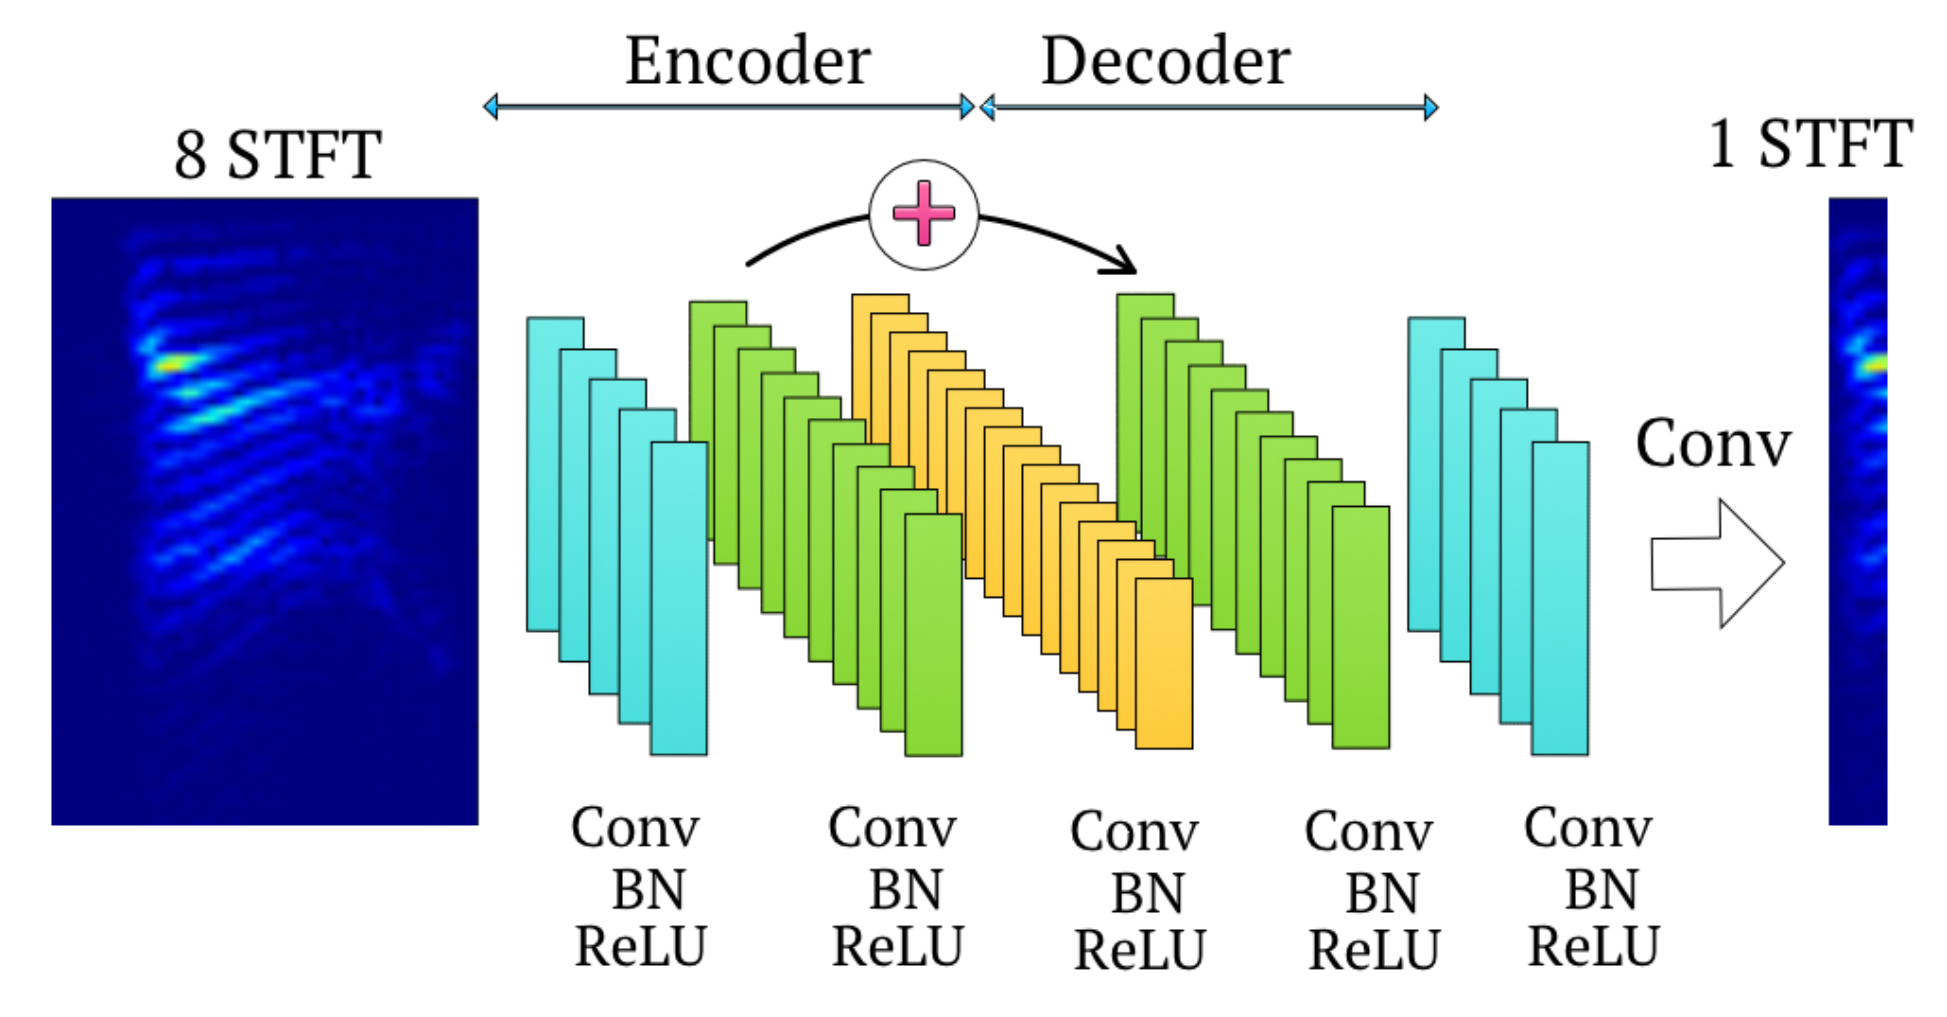
\includegraphics[width=\textwidth,keepaspectratio]{r-ced.png}
    \caption{\label{fig:rced}Redundant Convolutional Encoder Decoder (R-CED) architecture \cite{park2017acoustic}.}
\end{figure}

The R-CED architecture comprises a series of convolutional layers applied in sequence, with no intermediate pooling or upsampling operations. The convolution blocks are similar to those in the CED model. These are stacked symmetrically around the center of the network, forming a deep pipeline of transformations that preserve the input’s resolution at each stage.

The key innovation in the R-CED model is the use of redundant convolutional layers. Multiple layers with matching input and output dimensions, serve to increase the network’s capacity without reducing the temporal fidelity of the signal. According to the authors, this redundant structure helps the model learn more complex transformations over the same resolution domain, enabling superior denoising performance without sacrificing the granularity of spectrogram features.

The final convolutional layer is the same as in the CED model, with a large vertical kernel size of \(129 \times 1\) and a Tanh activation function. Projecting the output to two channels representing the denoised real and imaginary spectrogram components.

In contrast to both the baseline CNN and the CED model, the R-CED does not compress or expand the temporal resolution of the data. Instead, it relies entirely on the expressive capacity of multiple convolutional layers to model the mapping from noisy to clean spectrogram representations. This makes R-CED particularly suitable for applications where retaining precise time-frequency alignment is critical. In this project, the R-CED model is evaluated as a lightweight yet expressive alternative to deeper encoder-decoder variants.

\subsection{U-Net}
\label{sec:unet}

The U-Net model implemented in this project is adapted from the well-established U-Net architecture originally developed for biomedical image segmentation. In this work, the model is repurposed for complex spectrogram input handling and learns to generate a denoised spectrogram through a fully convolutional encoder-decoder structure with skip connections \cite{ronneberger2015unet}.

The core structure of U-Net is symmetric, comprising five downsampling stages (encoder), a bottleneck layer, and five upsampling stages (decoder). Each encoder block consists of a convolutional layer followed by instance normalization and a PReLU activation. Instance normalization is chosen over batch normalization to provide improved memory efficiency and stability when dealing with variable-length or low-batch-size audio inputs. The convolutional blocks downsample the features to a final latent representation of 1024 channels, which is then passed to the bottleneck layer.

\begin{figure}[h]
    \centering
    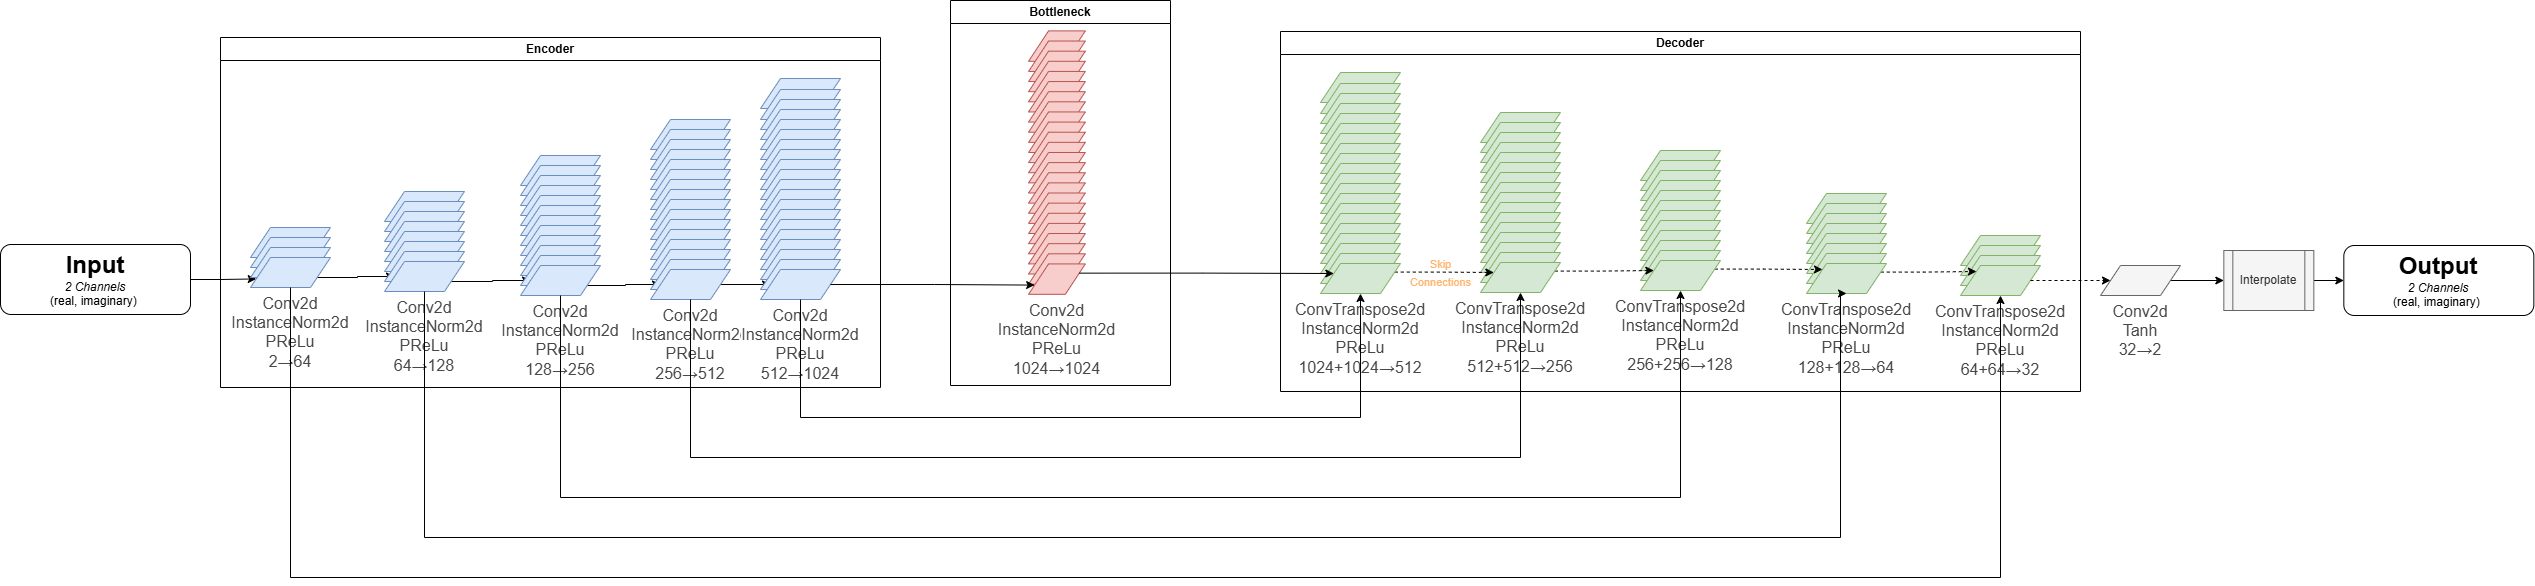
\includegraphics[width=\textwidth]{unet.png}
    \caption{\label{fig:unet}U-Net architecture used for complex spectrogram enhancement.}
\end{figure}

The bottleneck acts as the central transformation layer in the model. It comprises a single convolutional block with 1024 input and output channels, preserving the depth of the latent representation while providing non-linear transformation capabilities. Unlike traditional bottleneck layers that reduce dimensionality, this layer serves as a deep transformation point prior to decoding, facilitating high-capacity feature extraction.

The decoder mirrors the encoder with five upsampling blocks, each using transposed convolutions to increase resolution and reduce channel depth. Skip connections from corresponding encoder blocks are concatenated at each stage, preserving low-level features lost during downsampling. Each concatenated feature map is then processed with transposed convolutions, instance normalization, and PReLU activation, enhancing the model's ability to retain fine spectro-temporal details. The final decoder block reduces the output to 32 channels, followed by a $3 \times 3$ convolution projecting to two channels (real and imaginary). Final normalization and bilinear interpolation ensure the output size matches the original input dimensions.

This implementation of U-Net preserves the key architectural principles of the original model while tailoring it for speech enhancement. The use of instance normalization, PReLU activations, skip connections, and a deeper encoder-decoder path provides the network with strong representational power, allowing it to effectively recover clean speech from noisy spectrograms.


\subsection{Conv-TasNet}
\label{sec:convtasnet}

The Conv-TasNet model implemented in this project is based on the architecture proposed by Luo and Mesgarani~\cite{luo2019conv}, as discussed in Section~\ref{sec:convtasnet_lit_review}. Although the core structure is preserved, rigorous adaptations were required to align the model with the spectrogram-based framework used throughout this system.

The primary adaptation concerns the input format. While the original Conv-TasNet operates directly on raw time-domain waveforms, here the model is modified to process complex-valued spectrogram inputs. The real and imaginary parts are concatenated to form a two-channel input, which is passed through a \(3 \times 3\) convolutional encoder. The encoder maps the input to a latent space of 128 channels, using dynamic padding to maintain spatial dimensions.

\begin{figure}[h]
    \centering
    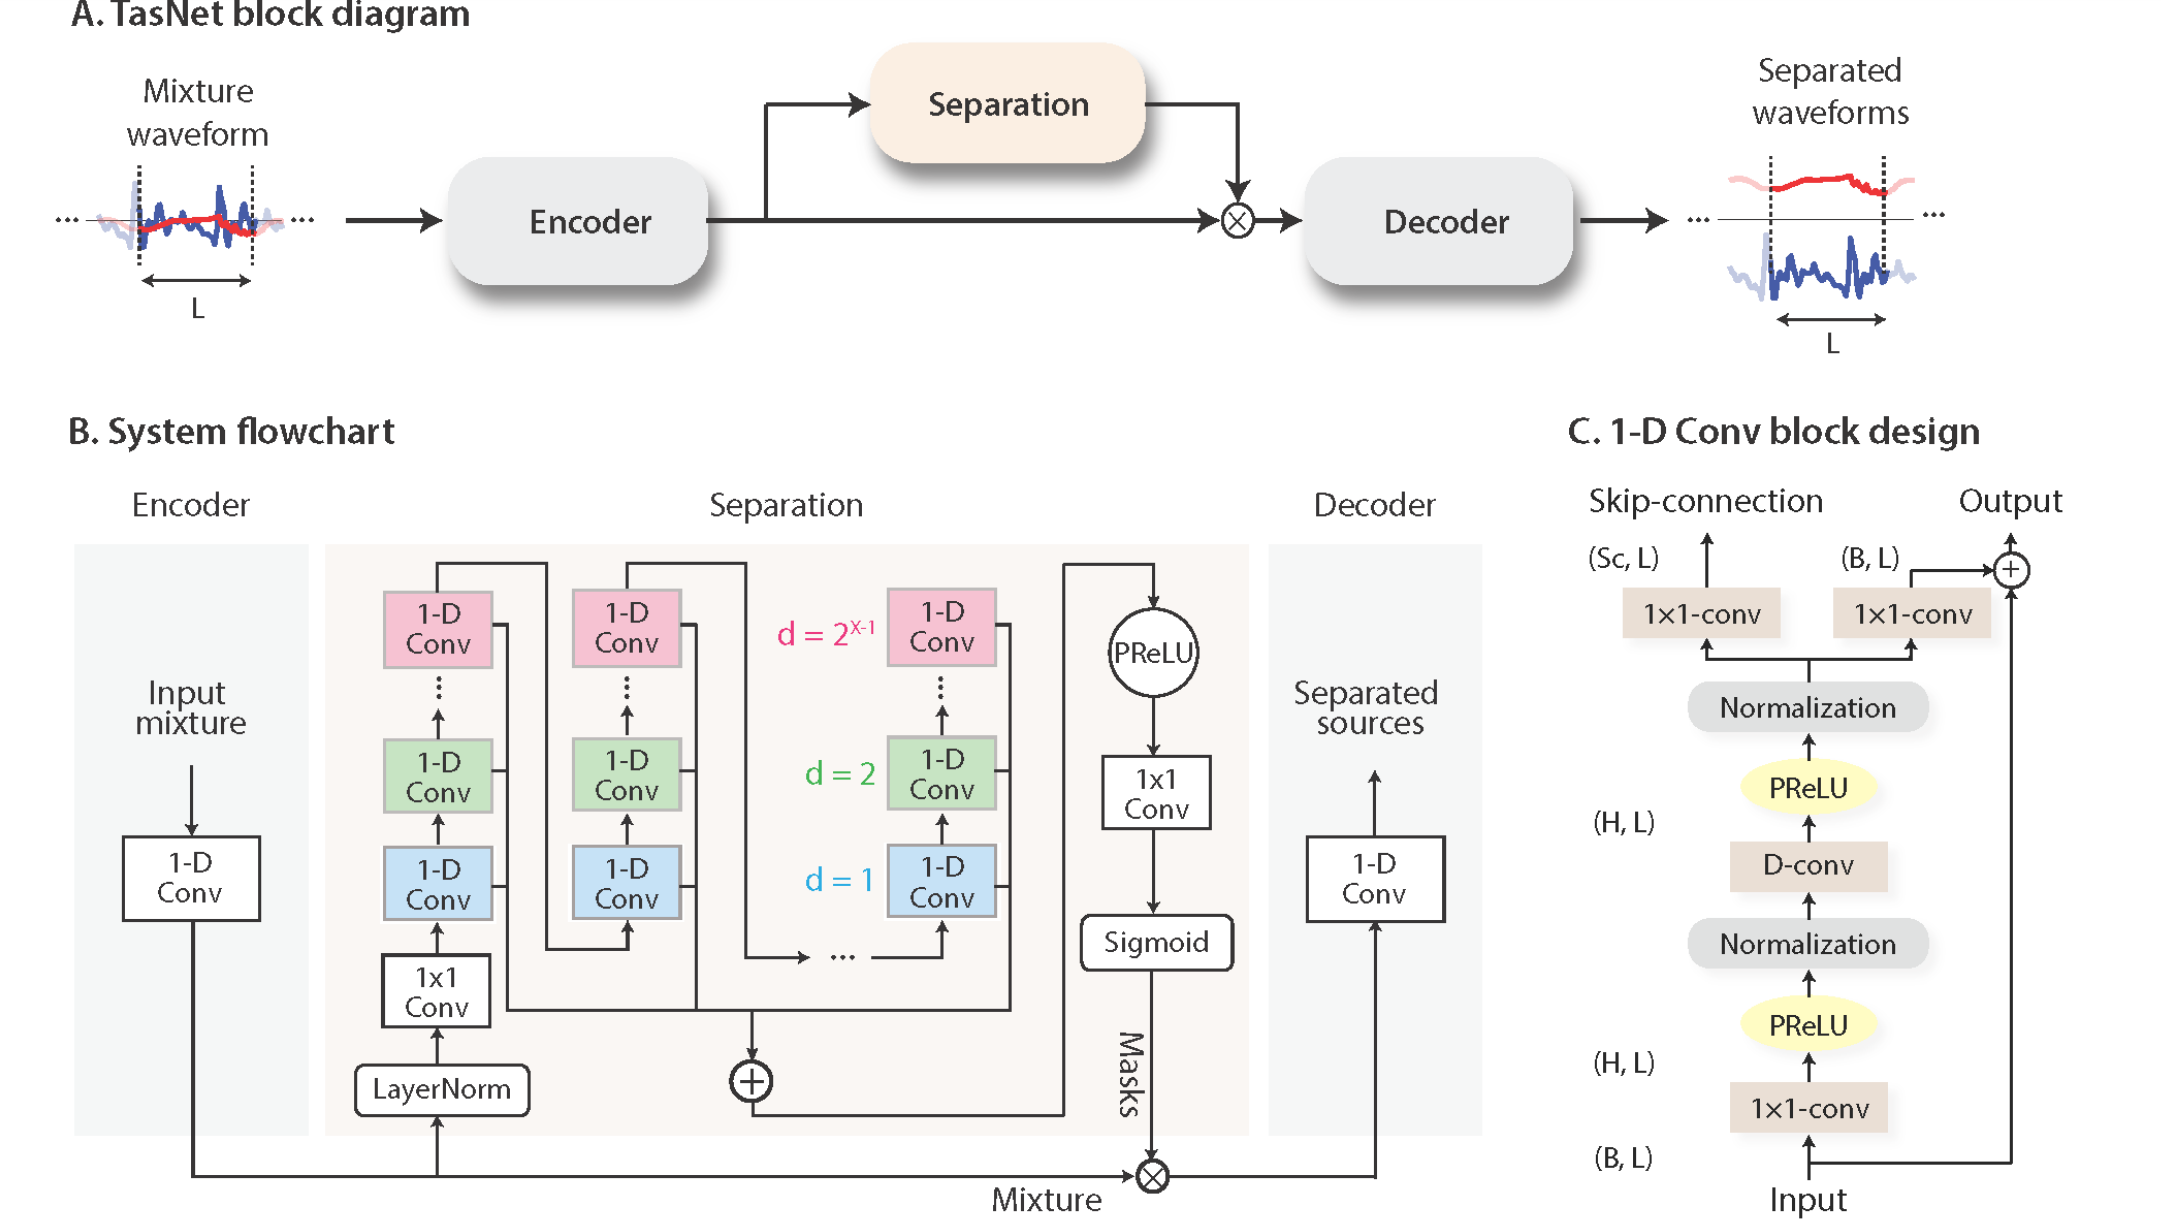
\includegraphics[width=\textwidth,keepaspectratio]{conv-tasnet.png}
    \caption{\label{fig:convtasnet}Conv-TasNet architecture overview \cite{luo2019conv}.}
\end{figure}

The latent representation is processed by the Temporal Convolutional Network (TCN), which forms the core of the separation module. The TCN consists of two stacks, each containing four residual blocks. Each residual block applies a \(3 \times 3\) convolution, followed by group normalization with eight groups, a PReLU activation, and a second convolution projecting back to the input dimension. Skip connections are used within each block to facilitate stable training and allow the network to capture long-range temporal dependencies efficiently.

One notable departure from the original Conv-TasNet design is the handling of output masking. While the original paper strongly emphasizes time-frequency masking, preliminary experiments in this project showed that implementing complex masking introduced significant architectural complexity and only resulted in marginal improvements in denoising performance. As a result, direct spectrogram enhancement without explicit masking was adopted to maintain simplicity.

Following the separation network, a \(3 \times 3\) convolutional decoder projects the latent features back to two output channels corresponding to the denoised real and imaginary spectrogram components. As in the encoder, dynamic padding ensures consistent output dimensions. Minor discrepancies between input and output sizes, due to cumulative convolutional padding effects, are corrected by cropping to align the final output with the original input dimensions before applying the inverse STFT.

This design adaptation preserves the core strength of Conv-TasNet, efficient temporal modeling through dilated convolutions, while enabling it to operate effectively on spectrogram-domain representations for speech denoising tasks.

\vspace{2em}

This project explores a range of neural network architectures for speech enhancement, beginning with a simple CNN-based autoencoder as a baseline. It then progresses to more advanced models such as the Convolutional Encoder Decoder (CED) and Redundant CED (R-CED), based on the work of Park and Lee~\cite{park2017acoustic}, which introduce deeper hierarchies and redundancy while preserving resolution.

The U-Net further improves performance through skip connections and a deep encoder-decoder design. While the Conv-TasNet~\cite{luo2019conv}, originally developed for speech separation, is adapted to operate on complex-valued spectrograms for denoising.

Together, these models provide a diverse and comparative landscape of machine learning approaches, highlighting architectural trade-offs and establishing strong baselines for benchmarking against classical signal processing methods.



